\documentclass[11pt]{article}

% --------------------------------------------------
% Packages
% --------------------------------------------------
\usepackage[margin=1in]{geometry}
\usepackage{amsmath, amssymb, amsthm}
\usepackage{mathtools}
\usepackage{graphicx}
\usepackage{float}
\usepackage{enumitem}
\usepackage{hyperref}
\usepackage{xcolor}
\usepackage{tikz}
\usetikzlibrary{arrows.meta, positioning, calc}

% Pseudocode and algorithms
\usepackage{algorithm}
\usepackage{algpseudocode}

% Better fonts (optional)
\usepackage{lmodern}

% --------------------------------------------------
% Hyperref setup
% --------------------------------------------------
\hypersetup{
    colorlinks=true,
    linkcolor=blue,
    citecolor=blue,
    urlcolor=blue
}

% --------------------------------------------------
% Theorem-like environments
% --------------------------------------------------
\theoremstyle{definition}
\newtheorem{definition}{Definition}[section]
\newtheorem{theorem}{Theorem}[section]
\newtheorem{claim}{Claim}[section]
\newtheorem{remark}{Remark}[section]

\theoremstyle{proof}
% Proof environment is built-in via amsthm

% --------------------------------------------------
% Custom commands
% --------------------------------------------------
\newcommand{\Gen}{\mathsf{Gen}}
\newcommand{\Enc}{\mathsf{Enc}}
\newcommand{\Dec}{\mathsf{Dec}}
\newcommand{\Sig}{\mathsf{Sig}}
\newcommand{\Ver}{\mathsf{Ver}}
\newcommand{\negl}{\mathsf{negl}}

% --------------------------------------------------
% Document
% --------------------------------------------------
\begin{document}

\title{Public Key Crypto notes - 06}
\author{By contributors}
\date{March 16. 2026}
\maketitle

\section{Proof of knowledge protocols}

\begin{itemize}
	\item Goal: Design a signature scheme that utilises the discrete log problem.
	\item Idea: Digital signature: Proof of knowledge of secret key without telling any information about it.
	\item Example: Ali Baba's cave: Bob can only pass meet Alice from $A$ when entering from $B$ if he knows the password. Alice does not hear the password.
	\item The probability of passing is 50\%. If Bob passes the test two times, 25\%, etc.
	\item Given $n$ tests, Bob can pass the test by randomly guessing with $\frac{1}{2^n}$ probability.
	\item This is a proof to the validator, Alice. For outside observers, no one can tell whether Bob really knows the password.
	\item Three steps:
	\begin{enumerate}
		\item Commitment: When the prover makes an action (Bob enters the cave).
		\item Challenge: When the validator asks the direction from Bob (\emph{”Enter from A and go through B”}).
		\item Response: When Bob comes from the corresponding direction.
	\end{enumerate}
\end{itemize}

\begin{figure}[H]
	\centering
	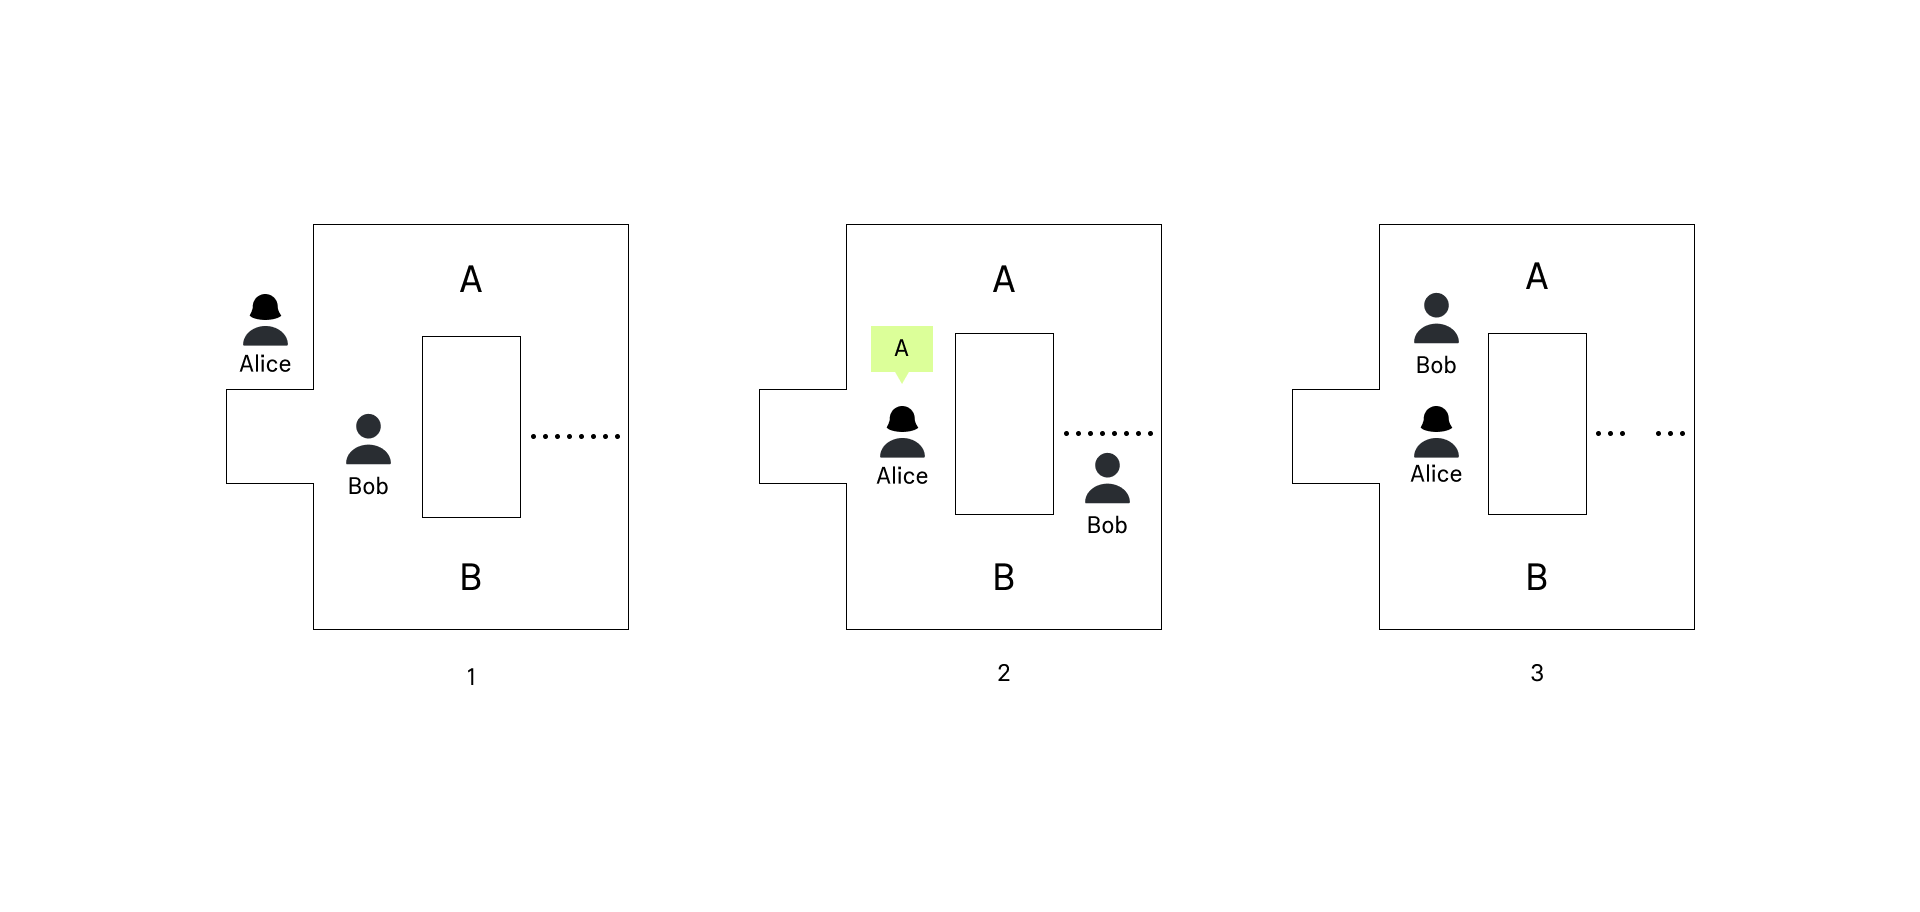
\includegraphics[width=0.7\textwidth]{images/ali_baba_cave.png}
	\caption{Ali Baba cave example}
	\label{fig:ali-baba}
\end{figure}

\subsection{Schnorr identification scheme}

Let $pk = (p, g, q, h=g^x), sk = x$.

\begin{itemize}
	\item Goal: Prove the knowledge of $sk$ under $pk$ without revealing any information on $sk$.
	\item Protocol:
	\begin{enumerate}
		\item Prover chooses $k \in_R \mathbb{Z}_q$ and $I=g^k$ and sends $I$ to the verifier. (Commitment)
		\item Verifier chooses $r \in_R \mathbb{Z}_q$ and sends this to the Prover. (Challenge)
		\item Prover computes $s=rx + k$ and sends $s$ to the  Verifier. (Response)
		\item Verifier checks: $I = g^s \cdot h^{-r}$. If yes, the proof is accepted.
	\end{enumerate}
	\item Correctness: $g^s \cdot h^{-r} = g^{rx + k} \cdot (g^x)^{-r} = g^{rx + k - rx} = g^k = I$
	
\end{itemize}

\begin{theorem}
	If the Prover can give a valid response for any challenge, then the Prover knows $x$.
\end{theorem}

\begin{proof}
	Let $I = g^k$ and let $r_1, r_2$ be two \emph{different} challenges with respect to $I$ and let $s_1, s_2$ be the two responses.
	
	\begin{align}
		s_1 &= r_1x + k \\
		s_2 &= r_2x + k \\
		s_1 - s_2 &= (r_1 - r_2)x \\
	\end{align}
	
	So:
	
	$$
	x = \frac{s_1 - s_2}{r_1 - r_2}
	$$
	
\end{proof}

\begin{remark}
	If the Prover knows $r$ in advance (before the commitment), they can generate a valid response $s$ without knowing secret $x$.
	
	\noindent Indeed: For a given challenge $r$, let $s \in_R \mathbb{Z}_q$ and $I = g^s \cdot g^{-r}$.
\end{remark}

Note that this is an interactive protocol, since the Verifier challenges the Prover. The Verifier's role is to generate the challenge. How can we make it non-interactive?

\subsection{Fiat-Shamir transform}

Replace the challenge $r$ with $r = H(I)$, where $H$ is a secure cryptographic hash function.

\noindent To prove security, we use the Random Oracle Model (ROM), where $H(.)$ is replaced by a random oracle.

\begin{definition}[Random Oracle Model (ROM)]
	For a given input $x$, if it has not been queried, then let $r \in_R \mathbb{Z}_q$, and put $r = \mathcal{O}(x)$, where $\mathcal{O}$ is the random oracle. If it has been queried, return the same output.
\end{definition}

\subsection{Schnorr signature scheme}

\begin{itemize}
	\item $\Gen$:
	\begin{itemize}
		\item Input: $1^n$
		\item Output: $pk = (p, g, q, h = g^x), sk = x$
	\end{itemize}
	\item $\Sig$:
	\begin{itemize}
		\item Input: $sk, m$
		\item Output: $(I, s)$, where:
		\begin{align}
			k &\in_R \mathbb{Z}_q, \\
			I &= g^k, \\
			r &= H(I, m), \\
			s &= rx + k
		\end{align}
	\end{itemize}
	\item $\Ver$:
	\begin{itemize}
		\item Input: $pk, m, (I, s)$
		\item Output: Compute $r = H(I, m)$ and check whether $I = g^s \cdot h^{-r}$
	\end{itemize}
\end{itemize}

\begin{theorem}
	The Schnorr signature scheme is secure, provided that $H(.)$ is modelled as a random oracle and the discrete logarithm problem is computationally hard.
\end{theorem}

\begin{proof}
	The proof uses the rewind technique. We prove by reduction. Assume we have a PPT adversary $A$ who can generate valid signatures with non-negligible probability. We use this $A$ to compute the discrete logarithm.
	
	For simplicity, we assume that $A$ is \emph{perfect}, meaning that it \emph{always} returns a valid signature.
	
	\noindent Reduction: Given $pk = (p, g, q, h = g^x)$. Our goal is to learn $x$. TODO: Ábra a füzetben
	
	\begin{enumerate}
		\item Give $pk$ to $A$.
		\item Give $A$ oracle access to $\mathcal{O}$, and let $Q$ be the set of queries submitted by $A$.
		\item $A$ generates $I$ and $m$ with $(I, m) \not \in R$ and queries the output $r = \mathcal{O}(I, m)$.
		\item $A$ returns $(I, s)$.
	\end{enumerate}
	
	Now, rewind it to step 3. and get $(i, s', r')$ at step 4. We have valid $(r, s)$ and $(r', s')$, with the same $I$, i.e. $s = rx + k$ and $s' = r'x + k$ with some $k$, such that $I = g^k$.
	
	This means that we can compute $x$.
\end{proof}

\begin{remark}
	This signature algorithm has been patented (expired in 2010). Instead, NIST designed a new and free signature algorithm called Digital Signature Algorithm (DSA).
\end{remark}

\end{document}